\documentclass{article}
\usepackage[utf8]{inputenc}
\usepackage{tikz}
\usetikzlibrary{positioning}
\usetikzlibrary{shapes}

\begin{document}

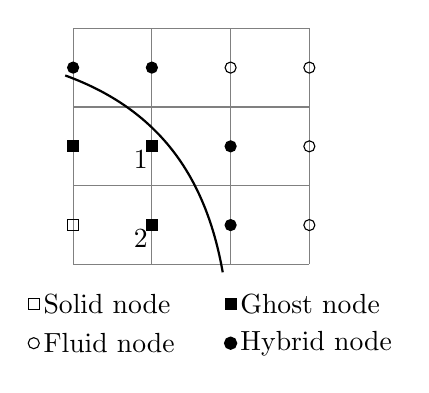
\begin{tikzpicture}
%grid
%horizontal
\draw[gray, thin] (-1.5,1.5) -- (1.5,1.5);
\draw[gray, thin] (-1.5,0.5) -- (1.5,0.5);
\draw[gray, thin] (-1.5,-0.5) -- (1.5,-0.5);
\draw[gray, thin] (-1.5,-1.5) -- (1.5,-1.5);
%vertical
\draw[gray, thin] (-1.5,1.5) -- (-1.5,-1.5);
\draw[gray, thin] (-0.5,1.5) -- (-0.5,-1.5);
\draw[gray, thin] (0.5,1.5) -- (0.5,-1.5);
\draw[gray, thin] (1.5,1.5) -- (1.5,-1.5);
%fluid nodes
\draw [black] (0.5,1) circle (2pt);
\draw [black] (1.5,1) circle (2pt);
\draw [black] (1.5,0) circle (2pt);
\draw [black] (1.5,-1) circle (2pt);
%hybrid nodes
\filldraw [black] (-1.5,1) circle (2pt);
\filldraw [black] (-0.5,1) circle (2pt);
\filldraw [black] (0.5,0) circle (2pt);
\filldraw [black] (0.5,-1) circle (2pt);
%body
\draw[black, thick] (-1.6,0.9) to[out=-20,in=100] (0.4,-1.6);
%ghost nodes
\filldraw ([xshift=-2pt,yshift=-2pt]-1.5,0) rectangle ++(4pt,4pt);
\filldraw ([xshift=-2pt,yshift=-2pt]-0.5,0) rectangle ++(4pt,4pt) node[anchor=north east] {1};
\filldraw ([xshift=-2pt,yshift=-2pt]-0.5,-1) rectangle ++(4pt,4pt) node[anchor=north east] {2};
%solid node
\draw ([xshift=-2pt,yshift=-2pt]-1.5,-1) rectangle ++(4pt,4pt);
%legend
\draw [black] (-2.0,-2.5) circle (2pt); 
\node[anchor=west] at (-2.0,-2.5) {Fluid node}; %fluid
\draw ([xshift=-2pt,yshift=-2pt]-2.0,-2.0) rectangle ++(4pt,4pt);
\node[anchor=west] at (-2.0,-2.0) {Solid node}; %solid
\filldraw ([xshift=-2pt,yshift=-2pt]0.5,-2.0) rectangle ++(4pt,4pt);
\node[anchor=west] at (0.5,-2.0) {Ghost node}; %ghost
\filldraw [black, thick] (0.5,-2.5) circle (2pt);
\node[anchor=west] at (0.5,-2.5) {Hybrid node};

\end{tikzpicture}


\end{document}
